\documentclass[10pt,letterpaper,final,twoside,notitlepage]{article}
\usepackage[margin=.5in]{geometry} % 1/2 inch margins on all pages
\usepackage[utf8]{inputenc} % Define the input encoding
\usepackage[USenglish]{babel} % Define language used
\usepackage{amsmath,amsfonts,amssymb}
\usepackage{amsthm} % Gives us plain, definition, and remark to use in \theoremstyle{style}
\usepackage{mathtools} % Allow for text and math in align* environment.
\usepackage{thmtools}
\usepackage{thm-restate}
\usepackage{graphicx}

\usepackage[
backend=biber,
style=alphabetic,
citestyle=authoryear]{biblatex} % Must include citation somewhere in document to print bibliography
\usepackage{hyperref} % Generate hyperlinks to referenced items
\usepackage[nottoc]{tocbibind} % Prints the Reference/Bibliography in TOC as well
\usepackage[noabbrev,nameinlink]{cleveref} % Fancy cross-references in the document everywhere
\usepackage{nameref} % Can make references by name to places
\usepackage{caption} % Allows for greater control over captions in figure, algorithm, table, etc. environments
\usepackage{subcaption} % Allows for multiple figures in one Figure environment
\usepackage[binary-units=true]{siunitx} % Gives us ways to typeset units for stuff
\usepackage{csquotes} % Context-sensitive quotation facilities
\usepackage{enumitem} % Provides [noitemsep, nolistsep] for more compact lists
\usepackage{chngcntr} % Allows us to tamper with the counter a little more
\usepackage{empheq} % Allow boxing of equations in special math environments
\usepackage[x11names]{xcolor} % Gives access to coloring text in environments or just text, MUST be before tikz
\usepackage{tcolorbox} % Allows us to create boxes of various types for examples
\usepackage{tikz} % Allows us to create TikZ and PGF Pictures
\usepackage{ctable} % Greater control over tables and how they look
\usepackage{diagbox} % Allow us to have shared diagonal cells in tables
\usepackage{multirow} % Allow us to have a single cell in a table span multiple rows
\usepackage{titling} % Put document information throughout the document programmatically
\usepackage[linesnumbered,ruled,vlined]{algorithm2e} % Allows us to write algorithms in a nice style.

\counterwithin{figure}{section}
\counterwithin{table}{section}
\counterwithin{equation}{section}
\counterwithin{algocf}{section}
\crefname{algocf}{algorithm}{algorithms}
\Crefname{algocf}{Algorithm}{Algorithms}
\setcounter{secnumdepth}{4}
\setcounter{tocdepth}{4} % Include \paragraph in toc
\crefname{paragraph}{paragraph}{paragraphs}
\Crefname{paragraph}{Paragraph}{Paragraphs}

% Create a theorem environment
\theoremstyle{plain}
\newtheorem{theorem}{Theorem}[section]
% Create a numbered theorem-like environment for lemmas
\newtheorem{lemma}{Lemma}[theorem]

% Create a definition environment
\theoremstyle{definition}
\newtheorem{definition}{Defn}
\newtheorem{corollary}{Corollary}[section]
% \begin{definition}[Term] \label{def:}
%   Make sure the term is emphasized with \emph{term}.
%   This ensures that if \emph is changed, it shows up everywhere
% \end{definition}

% Create a numbered remark environment numbered based on definition
% NOTE: This version of remark MUST go inside a definition environment
\theoremstyle{remark}
\newtheorem{remark}{Remark}[definition]
%\counterwithin{definition}{subsection} % Uncomment to have definitions use section.subsection numbering

% Create an unnumbered remark environment for general use
% NOTE: This version of remark has NO restrictions on placement
\newtheorem*{remark*}{Remark}

% Create a special list that handles properties. It can be broken and restarted
\newlist{propertylist}{enumerate}{1} % {Name}{Template}{Max Depth}
% [newlistname, LevelsToApplyTo]{formatting options}
\setlist[propertylist, 1]{label=\textbf{(\roman*)}, ref=\textbf{(\roman*)}, noitemsep, nolistsep}
\crefname{propertylisti}{property}{properties}
\Crefname{propertylisti}{Property}{Properties}

% Create a special list that handles enumerate starting with lower letters. Breakable/Restartable.
\newlist{boldalphlist}{enumerate}{1} % {Name}{Template}{Max Depth}
% [newlistname, LevelsToApplyTo]{formatting options}
\setlist[boldalphlist, 1]{label=\textbf{(\alph*)}, ref=\alph*, noitemsep, nolistsep} % Set options

\newlist{nocrefenumerate}{enumerate}{1} % {Name}{Template}{Max Depth}
% [newlistname, LevelsToApplyTo]{formatting options}
\setlist[nocrefenumerate, 1]{label=(\arabic*), ref=(\arabic*), noitemsep, nolistsep}

% Create a list that allows for deeper nesting of numbers. By default enumerate only allows depth=4.
\newlist{nestednums}{enumerate}{6}
% [newlistname, LevelsToApplyTo]{formatting options}
\setlist[nestednums]{noitemsep, label*=\arabic*.}

\tcbuselibrary{breakable} % Allow tcolorboxes to be broken across pages
% Create a tcolorbox for examples
% /begin{example}[extra name]{NAME}
% Create a tcolorbox for examples
% Argument #1 is optional, given by [], that is the textbook's problem number
% Argument #2 is mandatory, given by {}, that is the title for the example
% Avoid putting special characters, (), [], {}, ",", etc. in the title.
\newtcolorbox[auto counter,
number within=section,
number format=\arabic,
crefname={example}{examples}, % Define reference format for cref (No Capitals)
Crefname={Example}{Examples}, % Reference format for cleveref (With Capitals)
]{example}[2][]{ % The [2][] Means the first argument is optional
  width=\textwidth,
  title={Example \thetcbcounter: #2. #1}, % Parentheses and commas are not well supported
  fonttitle=\bfseries,
  label={ex:#2},
  nameref=#2,
  colbacktitle=white!100!black,
  coltitle=black!100!white,
  colback=white!100!black,
  upperbox=visible,
  lowerbox=visible,
  sharp corners=all,
  breakable
}

% Create a tcolorbox for general use
\newtcolorbox[% auto counter,
% number within=section,
% number format=\arabic,
% crefname={example}{examples}, % Define reference format for cref (No Capitals)
% Crefname={Example}{Examples}, % Reference format for cleveref (With Capitals)
]{blackbox}{
  width=\textwidth,
  % title={},
  fonttitle=\bfseries,
  % label={},
  % nameref=,
  colbacktitle=white!100!black,
  coltitle=black!100!white,
  colback=white!100!black,
  upperbox=visible,
  lowerbox=visible,
  sharp corners=all
}

% Redefine the 'end of proof' symbol to be a black square, not blank
\renewcommand{\qedsymbol}{$\blacksquare$} % Change proofs to have black square at end

% Common Mathematical Stuff
\newcommand{\Abs}[1]{\ensuremath{\lvert #1 \rvert}}
\newcommand{\DNE}{\ensuremath{\mathrm{DNE}}} % Used when limit of function Does Not Exist

% Complex Numbers functions
\renewcommand{\Re}{\operatorname{Re}} % Redefine to use the command, but not the fraktur version
\renewcommand{\Im}{\operatorname{Im}} % Redefine to use the command, but not the fraktur version
\newcommand{\Real}[1]{\ensuremath{\Re \lbrace #1 \rbrace}}
\newcommand{\Imag}[1]{\ensuremath{\Im \lbrace #1 \rbrace}}
\newcommand{\Conjugate}[1]{\ensuremath{\overline{#1}}}
\newcommand{\Modulus}[1]{\ensuremath{\lvert #1 \rvert}}
\DeclareMathOperator{\PrincipalArg}{\ensuremath{Arg}}

% Math Operators that are useful to abstract the written math away to one spot
% Number Sets
\DeclareMathOperator{\RealNumbers}{\ensuremath{\mathbb{R}}}
\DeclareMathOperator{\AllIntegers}{\ensuremath{\mathbb{Z}}}
\DeclareMathOperator{\PositiveInts}{\ensuremath{\mathbb{Z}^{+}}}
\DeclareMathOperator{\NegativeInts}{\ensuremath{\mathbb{Z}^{-}}}
\DeclareMathOperator{\NaturalNumbers}{\ensuremath{\mathbb{N}}}
\DeclareMathOperator{\ComplexNumbers}{\ensuremath{\mathbb{C}}}
\DeclareMathOperator{\RationalNumbers}{\ensuremath{\mathbb{Q}}}

% Calculus operators
\DeclareMathOperator*{\argmax}{argmax} % Thin Space and subscripts are UNDER in display

% Signal and System Functions
\DeclareMathOperator{\UnitStep}{\mathcal{U}}
\DeclareMathOperator{\sinc}{sinc} % sinc(x) = (sin(pi x)/(pi x))

% Transformations
\DeclareMathOperator{\Lapl}{\mathcal{L}} % Declare a Laplace symbol to be used

% Logical Operators
\DeclareMathOperator{\XOR}{\oplus}

% x86 CPU Registers
\newcommand{\rbpRegister}{\texttt{\%rbp}}
\newcommand{\rspRegister}{\texttt{\%rsp}}
\newcommand{\ripRegister}{\texttt{\%rip}}
\newcommand{\raxRegister}{\texttt{\%rax}}
\newcommand{\rbxRegister}{\texttt{\%rbx}}

%%% Local Variables:
%%% mode: latex
%%% TeX-master: shared
%%% End:


% These packages are more specific to certain documents, but will be availabe in the template
% \usepackage{esint} % Provides us with more types of integral symbols to use
% \usepackage{minted} % Allow us to nicely typeset 300+ programming languages

\graphicspath{./Drawings/Phys_224/} % Uncomment this to use pictures in this document

% This is the same as the remark environment. I need to go through subdocuments and remove
% \begin{note} and replace it with \begin{remark}
\theoremstyle{remark}
\newtheorem{note}{Note}[definition] % Note environment, counted by definition
\newtheorem*{note*}{Note}

% Math Operators that are useful to abstract the written math away to one spot
% These are supposed to be document-specific mathematical operators that will make life easier
% Many fundamental operators are defined in Reference_Sheet_Preamble.tex
\DeclareMathOperator{\PLD}{\text{PLD}}
\DeclareMathOperator{\Intensity}{I}

\begin{titlepage}
  \title{Phys 224: Modern Physics --- Reference Sheet \\ Illinois Institute of Technology}
  \author{Karl Hallsby}
  \date{Last Edited: \today}
\end{titlepage}

\begin{document}
\pagenumbering{gobble}
\maketitle
\pagenumbering{arabic}
\tableofcontents
\newpage
\pagenumbering{arabic}

\section{General Stuff}\label{sec:General}
\begin{itemize}[noitemsep]
\item Density: $\rho = \frac{\Delta m}{\Delta V}$
  \begin{itemize}
  \item Uniform Density: $\rho = \frac{m}{V}$
  \end{itemize}
\item Pressure: $p = \frac{\Delta F}{\Delta A}$
  \begin{itemize}
  \item Uniform Force on Flat Area: $\rho = \frac{F}{A}$
  \item Conversions: $1 atm = 1.01 \times 10^5 \si{\pascal} = 760 torr = 14.7 lb/in^2$
  \end{itemize}
\item Trig Relations are in \nameref{subsec:Trig Formulas}, Section~\ref{subsec:Trig Formulas}.
\end{itemize}

\section{Fluids} \label{sec:Fluids}
We must satisfy several parameters to make life easier, and to use most of these formulae.
	\begin{enumerate}[noitemsep]
		\item Incompressible - Density of the fluid is constant
		\item Non-turbulent Flow - Think of fluids swirling around an object
		\item Isostatic Pressure - Pressure inside the fluid is the same in all directions
	\end{enumerate}

	\begin{itemize}[noitemsep]
		\item Pressure at Some Depth - $p_{2} = p_{1} + \rho g \left( y_{1}-y_{2} \right)$
			\begin{itemize}
				\item Pressure at Depth $h \rightarrow p = p_{0} + \rho gh$
			\end{itemize}
		\item Pascal's Principle - 2 Parts
			\begin{enumerate}[noitemsep]
				\item $\vec{F_{o}} = \vec{F}_{i}\ \frac{A_{o}}{A_{i}}$
				\item $d_{o} = d_{i} \frac{A_{i}}{A_{o}}$
			\end{enumerate}
		\begin{itemize}[noitemsep, nolistsep]
			\item When 2 pressures should be equal, their forces are inversely proportional
			\item Set each pressure equal to each other, then solve for the missing variable.
		\end{itemize}
		\item Archimedes' Principle - $\vec{F}_{Up} = \vec{F}_{Down}$
			\begin{itemize}[noitemsep]
				\item Usually breaks down to $\vec{F}_{Bouyant} = \vec{F}_{g, Object}$
				\item $\vec{F}_{Bouyant} = m_{Object}g$
				\item $\vec{F}_{Bouyant} = \rho_{Object}V_{Object}g$
			\end{itemize}
		\item Continuity of Fluids
		\begin{itemize}[noitemsep]
			\item $A_{1}v_{1} = A_{2}v_{2}$
		\end{itemize}
		\item Bernoulli's Equation - $p_{1} + \frac{1}{2} \rho v_{1}^{2} + \rho gy_{1} = p_{2} + 	\frac{1}{2} \rho v_{2}^{2} + \rho gy_{2}$
			\begin{itemize}[noitemsep]
				\item Fluids at Rest - $p_{2} = p_{1} + \rho g \left( y_{1}-y_{2} \right)$
				\item Fluids not Changing Height - $p_{1} + \frac{1}{2} \rho v_{1}^{2} = p_{2} + 	\frac{1}{2} \rho v_{2}^{2}$
			\end{itemize}
	\end{itemize}

\section{Waves} \label{sec:Waves}
{\Large Usually of form $y = y_{m} \sin \left( kx \pm \omega t \right)$}
There are two types of waves:
	\begin{enumerate}[noitemsep, nolistsep]
		\item Transverse Waves - Waves where displacement from equilibrium is orthogonal to direction of propagation
		\begin{itemize}[noitemsep, nolistsep] % Examples of Transverse Waves
			\item String Waves
			\item Electromagnetic Waves
		\end{itemize}
		\item Longitudinal Waves - Waves where displacement from equilibrium is parallel to direction of propagation
		\begin{itemize}[noitemsep, nolistsep] % Examples of Longitudinal Waves
			\item Pressure Waves
			\item Sound Waves (Which are a type of pressure wave)
		\end{itemize}
	\end{enumerate}

	\begin{itemize}[noitemsep]
		\item $y_{m}$ - Amplitude, $m$
		\item $k$ - Angular Wave Number, $rad/m$
			\begin{itemize}[noitemsep, nolistsep]
				\item $k = \frac{2 \pi}{\lambda}$
				\item $\lambda$ is wavelength, $m$
			\end{itemize}
		\item $\omega$ - Angular Frequency, $rad/s$
			\begin{itemize}[noitemsep, nolistsep]
				\item $\omega = 2 \pi f$
				\item $f$ is frequency, $Hz$
				\item Sign of this goes the opposite the direction the wave is going
					\begin{enumerate}[noitemsep]
						\item Wave going in positive direction $\left( + \right)$, then the sign should be negative $\left( - \right)$
						\item Wave going in negative direction $\left( - \right)$, then the sign should be positive $\left( + \right)$
					\end{enumerate}
			\end{itemize}
		\item $v = \lambda f$, Wave Velocity, $m/s$
			\begin{itemize}[noitemsep]
				\item $v = \frac{\omega}{2 \pi} * \frac{2 \pi}{k} = \frac{\omega}{k}$
				\item This can be proven with the angular portion of any wave (inside the parentheses of trig function)
				\begin{align*} % Prove why k = \lambda / 2 \pi
					kx-\omega t &= \text{Constant} \\
					\frac{d}{dt} \left[ kx-\omega t \right] &= \frac{d}{dt} \left[ \text{Constant} \right] \\
					k \frac{dx}{dt} - \omega \frac{dt}{dt} &= 0 \\
					kv - \omega &= 0 \\
					kv &= \omega \\
					v &= \frac{\omega}{k} \\
				\end{align*}
				Since $\omega = 2 \pi f$ , then $k = \frac{\lambda}{2 \pi}$ 
			\end{itemize}
	\end{itemize}

	\subsection*{Wave Interference} \label{subsec:Wave Interference}
	Waves are nice, and they just sum when they interfere. Let: 
	\begin{align}
		y_{1} \left( x, t \right) &= y \sin \left( kx - \omega t \right) \\
		y_{2} \left( x, t \right) &= y \sin \left( kx + \omega t + \varphi \right) \\
		Y \left( x, t \right) &= y\left[ \sin \left( kx - \omega t \right) + \sin \left( kx + \omega t + \varphi \right) \right] \label{eq:Sum of 2 Waves}
	\end{align}
	You can usually use Equation~\ref{eq:Sin plus Sin with diff Angles} to simplify Equation~\ref{eq:Sum of 2 Waves}.

		\subsubsection*{Constructive/Destructive Interference} \label{subsubsec:Constructive/Destructive Interference}
		\begin{align*}		
			\phi &= 2 \pi \frac{Path Length Diff}{\lambda} = 2 \pi \frac{\Delta \text{PLD}}{\lambda} \\
			n &= \frac{\phi}{2\pi} = 4 \frac{Path Length Diff}{\lambda}\\
		\end{align*}
		\begin{itemize}[noitemsep]
			\item $Path Length Diff$ - Is the Difference in path lengths that the waves must travel
			\item $phi$ - Angular Location of points of Complete Constructive/Destructive Interference
			\item $n$ - Number of locations where there is Complete Constructive/Destructive Interference
		\end{itemize}

	\subsection*{Standing Waves} \label{subsec:Standing Waves}
	This is actually the superposition of 2 waves, traveling in opposite directions, on a medium that is fixed at both ends, i.e. a taut string held by a wall.
		\subsubsection*{Location of Nodes and Antinodes} \label{subsubsec:Node/Antinode Location}
		\begin{itemize}[noitemsep]
			\item Nodes - $x = n \frac{\lambda}{2}$ for $n = 0, 1, 2, \ldots$
			\begin{itemize}[noitemsep, nolistsep]
				\item Always at closed ends of tubes
			\end{itemize}
			\item Antinodes - $x = \left( n + \frac{1}{2} \right) \frac{\lambda}{2}$ for $n = 0, 1, 2, \ldots$
			\begin{itemize}[noitemsep, nolistsep]
				\item Always at open ends of tubes
			\end{itemize}
		\end{itemize}

		\subsubsection*{Resonant Frequencies/Harmonics} \label{subsubsec:Resonant Frequencies/Harmonics}
		These can also be called harmonics. There is a resonant frequency for every number of nodes/antinodes on tthe standing wave. \newline
		$f = \frac{v}{\lambda} = n \frac{v}{2L}$
		\begin{itemize}[noitemsep]
			\item $L$ is the length of the medium (The String).
			\item $\lambda$ is the wavelength of the wave formed.
		\end{itemize}
		This can be extended to find the base resonant frequency, if you know how many node levels are between the two resonant frequencies given, i.e. they say that the \textbf{NEXT} frequency, means $n+1$. \newline
		$f_{n+m}-f_{n} = \left( n+m \right) \frac{v}{2L} - n \frac{v}{2L} = m \frac{v}{2L}$
		
	\subsection*{Reflecting Sound} \label{subsec:Reflecting Sound}
		\begin{itemize}[noitemsep]
			\item $D = \left( n + 1 \right)d = vt$
			\begin{itemize}[noitemsep,nolistsep]
				\item $n$ is the number of reflections that occurred
				\item $n+1$ is used when we want the distance the wave covers
			\end{itemize}
		\end{itemize}
	
	\subsection*{Sound in Different Mediums} \label{subsec:Sound in Different Mediums}
	Frequency is a property of a wave, and \textbf{CANNOT BE ALTERED.} This means that:
	\begin{align*}
		v &= \lambda f \\
		v_{Sound, Material 1} &= \lambda_{Material 1}f_{Unique, Material 1} \\
		v_{Sound, Material 2} &= \lambda_{Material 2}f_{Unique, Material 2} \\
		f_{Unique, Material 1} &= f_{Unique, Material 2} \\
		\frac{v_{Sound, Material 1}}{\lambda_{Material 1}} &= \frac{v_{Sound, Material 2}}{\lambda_{Material 2}} \\
	\end{align*}
	
	\subsection*{Doppler Effect} \label{subsec:Doppler Effect}
	{\Large $f' = f \frac{v \pm v_{D}}{v \pm v_{S}}$}
	\begin{itemize}[noitemsep]
		\item Moving \textit{\textbf{TOWARDS}} each other: Frequency Increase
		\item Moving \textit{\textbf{AWAY}} from each other: Frequency Decrease
		\item $f$ - Initial Frequency, \si{\hertz}
		\item $v$ - Sound Speed, \si{\meter / \second}
		\item $v_{D}$ - Detector Speed, \si{\meter / \second}
		\item $v_{S}$ - Source Speed, \si{\meter / \second}
		\item \textbf{For Numerator}:
			\begin{itemize}[noitemsep,nolistsep]
				\item If detector is moving towards the source, $+$
				\item If detector is moving away from the source, $-$
			\end{itemize}
		\item \textbf{For Denominator}:
			\begin{itemize}[noitemsep,nolistsep]
				\item If source is moving away from detector, $+$
				\item If source is moving towards the detector, $-$
			\end{itemize}
		\end{itemize}


\section{Thermodynamics} \label{sec:Thermo}
	\begin{definition}[Thermodynamics] \label{def:Thermo}
		\emph{Thermodynamics} is the study of energy transfer between two macroscopic bodies driven by temperature differences.
	\end{definition}
	\begin{definition}[Temperature] \label{def:Temperature}
		\emph{Temperature} is a direct measurement of internal energy of a system
	\end{definition}

	\subsection{Laws of Thermodynamics} \label{subsec:Thermo Laws}
		\begin{definition}[0th Law of Thermodynamics] \label{def:0th Law of Thermo}
			If 2 bodies, A and B are in thermal equilibrium with a third body ``T'', then they are in thermal equilibrium with each other.
		\end{definition}
		\begin{definition}[1st Law of Thermodynamics] \label{def:1st Law of Thermo}
			\begin{equation} \label{eq:1st Law of Thermo}
				\begin{aligned}
					dE_{Internal} &= dQ - dT \text{, } dQ \text{ and } dT \text{ are inexact	(path-dependent) differentials.} \\
					\Delta E_{Internal} &= Q-T \\
				\end{aligned}
			\end{equation}
			\begin{note} \label{note:1st Law of Thermo Special Cases}
				\textbf{Special Cases for the 1st Law of Thermodynamics}:
				\begin{enumerate}[noitemsep, nolistsep]
					\item Adiabatic Processes - $dE_{Int} = -dW$
					\begin{itemize}[noitemsep, nolistsep]
						\item No heat exchange
						\item Insulating
						\item Something happens too quickly for system to keep up
					\end{itemize}
					\item Isothermal Processes - $dT = 0 \rightarrow dE_{Int} = 0 \rightarrow dQ = dW$
					\item Isobaric Processes - $dW = pdV$, $p$(pressure) is constant
					\item Constant Volume - $W = 0$
					\item Cyclical Processes - $dE_{Int} = 0 \rightarrow dQ = dW$
					\begin{itemize}[noitemsep, nolistsep]
						\item You end a cycle with the same internal energy when the cycle started
					\end{itemize}
				\end{enumerate}
			\end{note}
		\end{definition}
		\begin{definition}[2nd Law of Thermodynamics] \label{def:2nd Law of Thermo}
			If a \emph{cyclical process occurs in a CLOSED system}, the entropy of the system increases for irreversible processes and remains constant for reversible processes. \textbf{IT NEVER DECREASES!!}
			\begin{align} \label{eq:2nd Law of Thermo}
				\Delta S &\geq 0 \\
				\Delta S &= \int_{a}^{b} \frac{dQ \left( T \right)}{T} 
			\end{align}
			\begin{note}
				\textbf{$\mathbf{\Delta S}$ is a state-function, meaning it is path-independent.}
			\end{note}
		\end{definition}
	
	\subsection{Heat and Work} \label{subsec:Heat/Work}
		\begin{itemize}[noitemsep, nolistsep]
			\item $dW = \vec{F} \cdot \vec{ds}$
			\item $\vec{F} = p \left( V, T \right) dV$
			\item $W = \int p \left( V, T \right) dV$
			\item $W = \frac{dQ}{dt}$
			\item $W = \frac{\Delta Q}{\Delta t}$
		\end{itemize}
	\emph{\textbf{Work done by thermal energy is path independent.}}

	\subsection{Thermal Expansion} \label{subsec:Thermal Expansion}
	Occurs because the ``springs'' between each of the atoms in a lattice have energy applied by Heat (Temperature Change).
		\begin{itemize}
			\item $\frac{\Delta L}{L_{0}} = \alpha \Delta T$ (One-Dimensional Expansion)
			\item $\frac{dL}{L_{0}} = \alpha dT$ (One-Dimensional Expansion)
			\begin{itemize}[noitemsep, nolistsep]
				\item $\alpha$ is a material-specific constant
			\end{itemize}
		\end{itemize}
	
	\subsection{Specific Heat/Heat Capacity} \label{subsec:Specific Heat/Heat Capacity}
		\begin{itemize}
			\item $C = \frac{dQ}{dT} \leftarrow$ Specific Heat
			\item $c = \frac{dQ}{mdT} \leftarrow$ Mass Specific Heat
		\end{itemize}
	
	\subsection{Heat of Phase Transitions} \label{subec:Heat Phase Transitions}
	This is a constant unique to the material and the phase transition it is going through.
	\begin{itemize}[nolistsep]
		\item $Q = Lm$
		\item $Q = \int_{m_{i}}^{m_{f}} L_{f} dm$
		\begin{itemize}[noitemsep, nolistsep]
			\item $l_{Fusion} = $ Heat required to turn things from \textbf{SOLID TO LIQUID}
			\item $l_{Vapor} = $ Heat required to turn things from \textbf{LIQUID TO GAS}
		\end{itemize}
	\end{itemize}

	\subsection{Conduction Heat Transfer} \label{subsec:Conduction Heat Transfer}
	\begin{equation} \label{eq:Conduction Heat Transfer}
		P_{Conduction} = \frac{\left( T_{H} - T_{C} \right)}{L} Ak
	\end{equation}
		\begin{itemize}[noitemsep, nolistsep]
			\item $L$ = Length
			\item $A$ = Cross-Sectional Area
			\item $k$ = Material's Thermal Conductivity
		\end{itemize}
	For multiple materials between 2 thermal reservoirs:
	\begin{itemize}[noitemsep, nolistsep]
		\item $P_{1} = P_{2} = \ldots = P_{n}$
		\item Heat will only flow as fast as the slowest thermal conductor
	\end{itemize}


\section{Kinetic Theory of Ideal Gases} \label{sec:Kinetic Theory of Ideal Gases}
	\begin{definition}[Ideal Gas] \label{def:Ideal Gas}
		An \emph{ideal gas} is a gas that obeys the ideal gas law.
		\begin{equation} \label{eq:Ideal Gas Law}
			pV = nRT \text{, } R \approxeq 8.31 \si{\joule / \mole~\kelvin}
		\end{equation}
	\end{definition}
	\begin{align} \label{eq:Total Internal Energy of Ideal Gas}
		E_{Internal} &= K_{Translate} + K_{Rotate} \\
		\Delta E_{Internal} &= \Delta K_{Translate} + \Delta K_{Rotate} 
	\end{align}
	\begin{equation} \label{eq:Vrms of Ideal Gas}
		v_{rms} = \sqrt{\frac{3RT}{M}} \text{ M=molar mass of gas}
	\end{equation}
	
	\subsection{Mean Free Path} \label{subsec:Mean Free Path of Ideal Gas}
		\begin{definition}[Mean Free Path]
			The \emph{mean free path}, $\lambda$ is the average distance traversed by a molecule between collisions.
			\begin{equation} \label{eq:Mean Free Path of Ideal Gas}
				\lambda = \frac{1}{\sqrt{2} \pi d^{2} \frac{N}{V}}
			\end{equation}
			Where:
			\begin{itemize}[noitemsep, nolistsep]
				\item $d$ is the diameter of the atoms, or distance between centers during collision (\si{\meter})
				\item $N$ is the number of molecules (\si{\mole})
				\item $V$ is the volume of gas being handled (\si{\liter})
				\item $\lambda$ is the wavelength, the same as in $v=f\lambda$
			\end{itemize}
			\begin{note}
				If all the particles, except 1 are stationary, then you can use:
				\begin{equation} \label{eq:Mean Free Path of Stationary Ideal Gas}
					\lambda = \frac{1}{\pi d^{2} \frac{N}{V}}
				\end{equation}
			\end{note}
		\end{definition}
	
	\subsection{Work Done by Ideal Gases} \label{subsec:Work Done By Ideal Gas}
		\subsubsection{Isothermally} \label{subsubsec:Work Done Isothermally}
			\begin{equation}
				\begin{aligned}
					W &= \int \vec{F} \vec{ds} \\
					W &= \int_{V_{1}}^{V_{2}} p \left( V,T \right) dV \\
					W &= \int_{V_{1}}^{V_{2}} \frac{nRT}{V} dV \\
					W &= nRT \int_{V_{1}}^{V_{2}} \frac{1}{V} dV \\
					W &= nRT \ln \left( \frac{V_{2}}{V_{1}} \right) \\
				\end{aligned}
			\end{equation}
		\subsubsection*{Constant Pressure} \label{subsubsec:Work Done Under Constant Pressure}
			\begin{equation}
				W = p \left(V_{final}-V_{init} \right)
			\end{equation}
			
	\subsection{Translational Kinetic Energy} \label{subsec:Translational Kinetic Energy}
		\begin{definition}[Degrees of Freedom] \label{def:Degrees of Freedom}
			\emph{Degrees of freedom} represent the number of variables that are needed to describe a system. Represented with $d$, occasionally.
			\begin{note}
				In an ideal gas, these are a means to store energy.
			\end{note}
		\end{definition}
		\begin{equation} \label{eq:Translational Kinetic Energy}
			\begin{aligned}
				K_{Translate} &= \frac{3}{2}nRT \\
				\Delta K_{Translate} &= \frac{3}{2}nR \Delta T \\
			\end{aligned}
		\end{equation}
		\begin{table}[h!]
			\centering
			\begin{tabular}{c|c|c|c}
				 & Translational & Rotational & Total \\ \hline
				Monatomic & 3 & 0 & 3 \\ \hline
				Diatomic & 3 & 2 & 5 \\ \hline
				Polyatomic & 3 & 3 & 6 \\
			\end{tabular}
			\caption{Degrees of Freedom Table for Gases}
			\label{tab:Degrees of Freedom}
		\end{table}
		\begin{itemize}[noitemsep, nolistsep]
			\item An ideal gas has \emph{\textbf{ONLY}} kinetic energy
			\item Completely elastic collisions
		\end{itemize}
		
		\begin{equation} \label{eq:Internal Energy of Ideal Gas}
			E_{int} = \frac{DoF}{2} nRT \text{, where } DoF=\text{Degrees of Freedom}
		\end{equation}
		
	\subsection{Molar Specific Heats of Ideal Gases} \label{subsec:Molar Specific Heats of Ideal Gases}
		\subsubsection{Molar Specific Heat @ Constant Volume} \label{subsubsec:Molar Specific Heat at Constant Volume}
			\begin{equation} \label{eq:Molar Specific Heat at Constant Volume}
				\begin{aligned}
					C_{V} &= \frac{\Delta E}{n \Delta T} \\
					C_{V} &= \frac{dE}{dT} \\
					C_{V} &= \left( \frac{DoF}{2} \right) R \\
				\end{aligned}
			\end{equation}
			\begin{equation} \label{eq:Heat with Molar Specific Heat at Constant Volume}
				Q = n C_{V} \Delta T
			\end{equation}
			
		\subsubsection{Molar Specific Heat @ Constant Pressure} \label{Molar Specific Heat at Constant Pressure}
			\begin{equation} \label{eq:Molar Specific Heat at Constant Pressure}
				C_{P} = C_{V} + R
			\end{equation}
			\begin{equation} \label{eq:Heat with Molar Specific Heat at Constant Pressure}
			Q = n C_{P} \Delta T
			\end{equation}
	
	\subsection{Adiabatic Processes in Ideal Gases} \label{subsec:Adiabatic Processes in Ideal Gases}
		\begin{definition}[Adiabatic Process] \label{def:Adiabatic Processes in Ideal Gases}
			An \emph{adiabatic process} is one in which no heat exchange occurs, namely:
			\begin{equation} \label{eq:Adiabatic Processes in Ideal Gases}
				\begin{aligned}
					dE_{Internal} &= dQ - dW \\
					dQ &= 0 \\
					dE_{Internal} &= -dW \\
				\end{aligned}
			\end{equation}
		\end{definition}
		This leads to:
		\begin{equation}
			pV^{\gamma} = \text{Constant}, \gamma = \frac{C_{P}}{C_{V}}
		\end{equation}
		\begin{equation} \label{eq:Adiabatic Pressure Volume}
			p_{1}V_{1}^{\gamma} = p_{2}V_{2}^{\gamma}
		\end{equation}
		\begin{equation} \label{eq:Adiabatic Temperature Volume}
			T_{1}V_{1}^{\gamma -1} = T_{2}V_{2}^{\gamma -1} 
		\end{equation}
		You get Equation~\eqref{eq:Adiabatic Temperature Volume} by plugging $p = \frac{nRT}{V}$ into Equation~\eqref{eq:Adiabatic Pressure Volume}.

\section{Entropy} \label{sec:Entropy}
There is a heavy relationship between this and the \nameref{def:2nd Law of Thermo}.
	\begin{definition}[Entropy] \label{def:Entropy}
		\emph{Entropy} is a measure of the number of available states/configurations.
		\emph{Entropy} can be thought of as a measure of the probability of an energy distribution in materials.
		Entropy states that energy will want ot end in its most probable state, where it is most event distributed.
		The \emph{units for entropy} are \si{\joule / \kelvin}.
		\begin{equation} \label{eq:Entropy}
			S = k_{B} \ln \left( \Omega \right)
		\end{equation}
		\begin{note}
			\textbf{Entropy is NOT disorder.}
		\end{note}
	\end{definition}
	\begin{definition}[Change in Entropy] \label{def:Change in Entropy}
		\emph{Change in entropy} is the change in the number of available states/configurations for energy in a system.
		\begin{equation} \label{eq:Change in Entropy}
			\begin{aligned}
				\Delta S &= S_{f} - S_{i} \\
						 &= \int_{a}^{b} \frac{dQ \left( T \right)}{T} \\
						 &= nR \ln \left( \frac{V_{f}}{V_{i}} \right) \\
						 &= mC \ln \left( \frac{T_{f}}{T_{i}} \right) \\
			\end{aligned}
		\end{equation}
		\begin{note}
			Because $\Delta S$ is based off of heat,
			\begin{equation}
				\Delta S_{Total} = \sum_{states} \Delta S
			\end{equation}
		\end{note}
	\end{definition}

	\subsection{Engines} \label{subsec:Engines}
	Engines are inherently cyclical.
		\begin{definition}[Efficiency] \label{def:Efficiency}
			\emph{Efficiency} is a measure of how effect an engine is in turning the heat taken in and turning it into work out.
			\begin{equation} \label{eq:Efficiency}
				\begin{aligned}
					\text{Efficiency} &= \frac{W_{Out}}{Q_{In}} \\
					\text{Eff} &= \frac{Q_{In}-Q_{Out}}{Q_{In}} \\
					\text{Eff} &= \frac{T_{Hot}-T_{Cold}}{T_{Hot}} \\
				\end{aligned}
			\end{equation}
		\end{definition}
	
		\subsubsection{Stirling Engine} \label{subsubsec:Stirling Engine}
		Based on the \nameref{eq:Ideal Gas Law}.
		You can find \nameref{def:Efficiency} with Equation~\eqref{eq:Efficiency}.
		
		\subsubsection{Carnot Engine} \label{subsubsec:Carnot Engine}
		Uses Isothermal expansion and adiabatic expansion of gases to achieve work.
		The total work done is the area of the Carnot figure.
		You can find \nameref{def:Efficiency} with Equation~\eqref{eq:Efficiency}.
		
			\begin{definition}[Coefficient of Performance] \label{def:Coefficient of Performance}
				\emph{Coefficient of performance} is a measurement of the amount of energy a Carnot engine moves in comparison to its cold reservoir.
				\begin{equation} \label{eq:Coefficient of Performance}
					\begin{aligned}
						K_{C} &= \frac{T_{L}}{T_{H} - T_{L}} \\
						K_{C} &= \frac{\lvert Q_{L} \rvert}{\lvert Q_{H} \rvert - \lvert Q_{L} \rvert} \\
						K &= \frac{\lvert Q_{L} \rvert}{\lvert W \rvert} \\
					\end{aligned}
				\end{equation}
			\end{definition}

\section{Light} \label{sec:Light}
	\begin{definition}[Photon]
		A \emph{photon} is an electric field (wave) propagating through another electric field.
	\end{definition}
The various $\theta$ used in Equations~\eqref{eq:Reflected Light},~\eqref{eq:Refracted Light} are measured from the surface normal.

\emph{Chromatic Dispersion} is the breaking up of polychromatic light by spectra.
Think of Pink Floyd's \textit{Dark Side of the Moon} album cover.
This happens because shorter wavelength, higher frequency light has a slightly higher index of refraction.
%	\begin{figure}[h!]
%		\centering
%		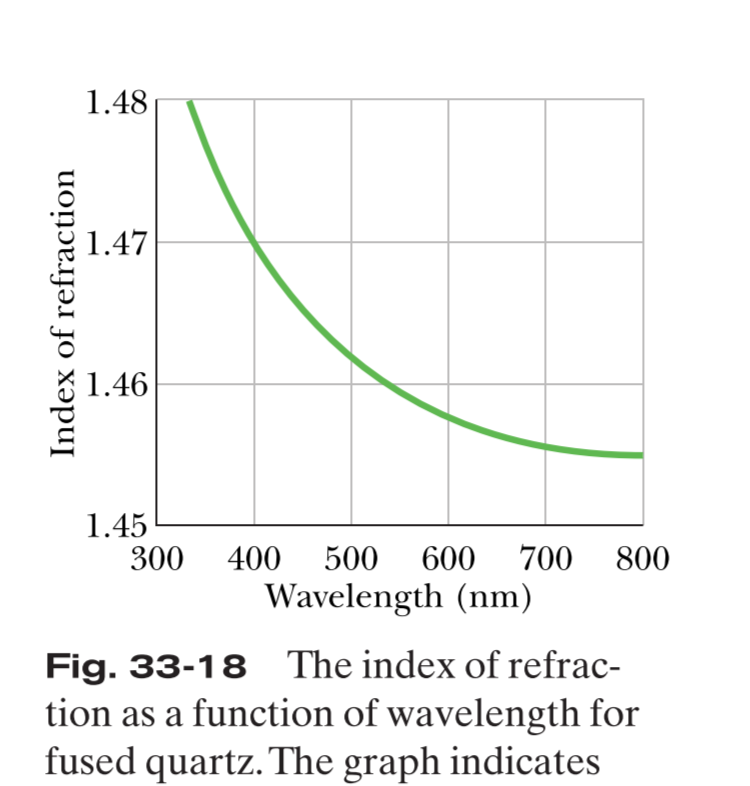
\includegraphics[scale=0.5]{Polychromatic_Light_Indices_Refraction.png}
%		\caption{Indices of Refraction for Polychromatic Light}
%		\label{fig:Indices of Refraction for Polychromatic Light}
%	\end{figure}

	\subsection*{Reflection} \label{subsec:Reflection}
		\begin{equation} \label{eq:Reflected Light}
			\theta_{reflected} = \theta_{incident}
		\end{equation}
		
	\subsection*{Refraction} \label{subsec:Refraction}
		\begin{definition}[Snell's Law] \label{def:Snell's Law}
			\begin{equation} \label{eq:Refracted Light} 
				n_{refract} \sin \left( \theta_{refract} \right) = n_{incident} \sin \left( \theta_{incident} \right)
			\end{equation}
		\end{definition}
		\begin{definition}[Index of Refraction] \label{def:Index of Refraction}
			\begin{equation} \label{eq:Index of Refraction}
				\begin{aligned}
					n_{i} &= \frac{c}{v_{i}} \\
					\lambda &= \frac{\lambda_{0}}{n} \\
				\end{aligned}
			\end{equation}
		\end{definition}
	
	\subsection*{Total Internal Reflection} \label{subsec:Total Internal Reflection}
		\begin{definition}[Total Internal Reflection] \label{def:Total Internal Reflection}
			Total Internal Reflection occurs when the \emph{refracted light's angle is $\frac{\pi}{2}$}.
			\begin{equation} \label{eq:Total Internal Reflection}
				n_{refract} \sin \left( \theta_{refract} \right) = n_{incident} \sin \left( \theta_{incident} \right) \text{, where } \theta_{refract} = \frac{\pi}{2}
			\end{equation}
		\end{definition}
		
	\subsection*{Interference and Diffraction} \label{subsec:Interference and Diffraction}
		\begin{definition}[Huygen's Principle] \label{def:Huygen's Principle}
			Any point on a plane wavefront can be treated as a source of outgoing spherical waves.
			\begin{note}
				This is a mathematical construct/model.
			\end{note}
		\end{definition}
		\begin{definition}[Phase Difference] \label{def:Phase Difference}
			Waves from the same source, but measured in such a way that there is a Path Length Difference (PLD) between them will have a \emph{phase difference}.
			\begin{equation} \label{eq:Phase Difference}
				\varphi = \frac{2 \pi \PLD}{\lambda}
			\end{equation}
		\end{definition}
	All \nameref{subsec:Interference and Diffraction} equations used from here on out are based on Equation~\eqref{eq:Phase Difference}.
		\begin{definition}[Single Slit Diffraction] \label{def:Single Slit Diffraction}
			When waves propagate through a single slit, there is a Probability Distribution Function that describes where intensity of light is greatest and smallest.
			The location of the \emph{\textbf{minima}} are given in Equation~\eqref{eq:Minima of Single Slit Diffraction}
			\begin{equation} \label{eq:Minima of Single Slit Diffraction}
				m \lambda = a \sin \left( \theta_{m} \right)
			\end{equation}
			\begin{note}
				$m$ is the number of minima from the central major distribution of intensity.
				\begin{enumerate}[noitemsep, nolistsep]
					\item First minima means $m=1$
					\item Second minima means $m=2$
					\item etc.
				\end{enumerate}
			\end{note}
			Thus, the equation for the \nameref{eq:Phase Difference of Single Slit Diffraction} is given in Equation~\eqref{eq:Phase Difference of Single Slit Diffraction}.
			\begin{equation} \label{eq:Phase Difference of Single Slit Diffraction}
				\varphi_{\text{Single Slit}} = \frac{2 \pi}{\lambda} a \sin \left( \theta \right)
			\end{equation}
		\end{definition}
		\begin{definition}[Double Slit Diffraction] \label{def:Double Slit Diffraction}
			This is really interference.
			The \emph{\textbf{maxima}} of the interference is given in Equation.
			\begin{equation} \label{eq:Maxima of Double Slit Diffraction}
				n \lambda = d \sin \left( \theta_{n} \right)
			\end{equation}
			\begin{note}
				$n$ is the number of maxima from the central major distribution of intensity.
				\begin{enumerate}[noitemsep, nolistsep]
					\item First maxima means $n=1$
					\item Second maxima means $n=2$
					\item etc.
				\end{enumerate}
			\end{note}
			Thus, the equation for the \nameref{eq:Phase Difference of Double Slit Refraction} is given in Equation~\eqref{eq:Phase Difference of Double Slit Refraction}.
			\begin{equation} \label{eq:Phase Difference of Double Slit Refraction}
				\varphi_{\text{Double Slit}} = \frac{2 \pi}{\lambda} d \sin \left( \theta \right)
			\end{equation}
		\end{definition}

\section{Quantum Mechanics} \label{sec:Quantum Mech}
Quantum mechanics may seem strange or weird, but it really isn't.
	\begin{definition}[Hamiltonian] \label{def:Hamiltonian}
		The \emph{hamiltonian} is a function that contains all knowable information about a particle or system in classical mechanics.
		\begin{equation} \label{eq:Hamiltonian}
			\text{Hamiltonian} = K+U
		\end{equation}
		\begin{itemize}[noitemsep, nolistsep]
			\item $K$ is the Kinetic Energy of the particle of system of particles.
			\begin{itemize}[noitemsep, nolistsep]
				\item $K = \frac{1}{2} mv^{2}$
				\item This contains the velocity of the system, which includes direction.
			\end{itemize}
			\item $U$ is the Potential Energy of the particle or system of particles.
			\begin{itemize}[noitemsep, nolistsep]
				\item $U = mg \left( y_{2} - y_{1} \right)$
				\item Contains the force of the system, its location, etc.
			\end{itemize}
		\end{itemize}
	\end{definition}

	\subsection{Schr\"{o}dinger's Equation} \label{subsec:Schrodingers Equation}
		\begin{definition}[de Broglie Wavelength] \label{def:de Broglie Wavelength}
			The \emph{de Broglie wavelength, $\lambda$}, is the wavelength that is \emph{associated} with a particle.
			In other words, a particle does \emph{\textbf{not}} have a wavelength, but the equations describing the particle's actions have a wavelength.
			\begin{note} \label{note:de Broglie Wavelength Momentum}
				As a direction consequence of the \nameref{def:de Broglie Wavelength},
				\begin{equation}
					p = \frac{h}{\lambda}
				\end{equation}
				\begin{itemize}[noitemsep, nolistsep]
					\item $h$ is Planck's Constant
					\item $\lambda$ is the \nameref{def:de Broglie Wavelength}
				\end{itemize}
			\end{note}
		\end{definition}
		\begin{definition}[Schr\"{o}dinger's Equation] \label{def:Schrodinger's Equation}
			\emph{Schr\"{o}dinger's equation} is a 3-dimensional Cartesian, time-independent way to express the equivalent of a \nameref{def:Hamiltonian} for quantum effects, namely in terms of waves (Denoted with $\Psi$).
			There are 2 equivalent ways to express \nameref{def:Schrodinger's Equation}.
			The first way, Equation~\eqref{eq:Schrodinger's Equation, Form 1}, is the most general form.
			The second way, Equation~\eqref{eq:Schrodinger's Equation, Form 2}, has expanded the nabla operator, $\nabla$.
			\begin{equation} \label{eq:Schrodinger's Equation, Form 1}
				\frac{- \hbar^{2}}{2m} \cdot \nabla^{2} \Psi + V\Psi = E\Psi
			\end{equation}
			\begin{equation} \label{eq:Schrodinger's Equation, Form 2}
				\frac{-\hbar}{2m} \left( \frac{\partial^{2} \Psi}{\partial x^{2}} + \frac{\partial^{2} \Psi}{\partial y^{2}} + \frac{\partial^{2} \Psi}{\partial z^{2}} \right) + V\Psi = E\Psi
			\end{equation}
			\begin{itemize}[noitemsep, nolistsep]
				\item $E$ is the \emph{\textbf{total}} energy of the system
				\item $V$ is the \emph{\textbf{potential energy}} of the system. It may be:
				\begin{enumerate}[noitemsep, nolistsep]
					\item Constant
					\item A function of time and/or space
				\end{enumerate}
				\item $\Psi$ is a solution to \nameref{def:Schrodinger's Equation}, and contains all that can be known about the system
				\item $\frac{-\hbar^{2}}{2m} \cdot \nabla\Psi$ is the \emph{\textbf{kinetic energy}} operator
				\begin{itemize}[noitemsep, nolistsep]
					\item $\nabla^{2} = \frac{\partial^{2}}{\partial x^{2}} + \frac{\partial^{2}}{\partial y^{2}} + \frac{\partial^{2}}{\partial z^{2}}$ is in the Cartesian coordinate system ($x$, $y$, $z$), and is called ``del squared'', or ``2nd-degree nabla.''
				\end{itemize}
				\item For each observable system, there exists a corresponding mathematical operator.
			\end{itemize}
			\begin{note} \label{note:Psi Probability Distribution Function of Particle Location}
				The probability distribution function of the position of a particle in the system can be found according to Equation~\eqref{eq:Psi Probability Distribution Function of Particle Location}.
				This is the multiplication of $\Psi$ with its complex conjugate, $\Psi^{*}$.
				\begin{equation} \label{eq:Psi Probability Distribution Function of Particle Location}
					\text{PDF} = \Psi \cdot \Psi^{*}
				\end{equation}
			\end{note}
		\end{definition}
		\subsubsection{Properties of Schr\"{o}dinger's Equation} \label{subsubsec:Properties of Schrodingers Equation}
			Solutions, $\Psi$, to \nameref{def:Schrodinger's Equation} have the following characteristics:
			\begin{enumerate}[noitemsep, nolistsep]
				\item They are single-valued
				\item They are piecewise continuous values
				\item $\frac{\partial \Psi}{\partial x}$, $\frac{\partial \Psi}{\partial y}$, $\frac{\partial \Psi}{\partial z}$ are all continuous
				\item $\iiint \Psi \Psi^{*} \partial x \partial y \partial z$ is square integrable, or $\iiint \Psi \Psi^{*} \partial x \partial y \partial z \neq \pm \infty$
			\end{enumerate}

		\begin{proof}[Rough Justification of \nameref{def:Schrodinger's Equation}] \label{proof:Schrodinger's Equation Justification}
		If $\Psi$ is to be a wave function, it must satisfy the following differential equation:
		\begin{equation*}
			\frac{\partial^{2} \Psi}{\partial x^{2}} = \frac{1}{v^{2}} \frac{\partial^{2} \Psi}{\partial t^{2}}
		\end{equation*}
		Since we are looking for \nameref{eq:Schrodinger's Equation, Form 1}, in which all the dynamical observables are contained within $\Psi$, we will set $v=c$, the upper limit of information transfer.
		We will first consider (without loss of generality) one dimension, the $x$-dimension.
		Then,
		\begin{equation*}
			\frac{\partial^{2} \Psi}{\partial x^{2}} = \frac{1}{v^{2}} \frac{\partial^{2} \Psi}{\partial t^{2}}
		\end{equation*}
		As a test solution, we will propose
		\begin{equation*}
			\Psi = A e^{-i \left( kx-\omega t \right)}
		\end{equation*}
		With respect to $x$:
		\begin{align*}
			\frac{\partial \Psi}{\partial x} &= A \left( -ik \right) e^{-i \left( kx-\omega t \right)} \\
			\frac{\partial^{2} \Psi}{\partial x^{2}} &= A \left( -ik \right)^{2} e^{-i \left( kx-\omega t \right)} = \left( -ik \right)^{2} \Psi = k^{2} \Psi \\
		\end{align*}
		Therefore, $\Psi$ is a satisfactory solution in $x$.
		With respect to $t$:
		\begin{align*}
			\frac{\partial \Psi}{\partial t} &= A \left( i\omega \right) e^{-i \left( kx-\omega t \right)} \\
			\frac{\partial^{2} \Psi}{\partial t^{2}} &= A \left( i\omega \right)^{2} e^{-i \left( kx-\omega t \right)} \\
		\end{align*}
		Therefore, $\Psi$ is a satisfactory solution in $t$.
		Thus, $\Psi$ is a solution to $\frac{\partial^{2} \Psi}{\partial x^{2}} = \frac{1}{c^{2}} \frac{\partial^{2} \Psi}{\partial t^{2}}$.
		(Also, $\frac{1}{c^{2}} = \frac{k^{2}}{\omega^{2}}$). \newline
		In our solution, $\Psi = A e^{-i \left( kx-\omega t \right)} $, k has its usual meaning:
		\begin{equation*} 
			k = \frac{2 \pi}{\lambda}
		\end{equation*}
		\emph{Where the wavelength, $\lambda$, is to be the \nameref{def:de Broglie Wavelength}, i.e. the wavelength that is associated with a particle.}
		In otherwords, a particle does not have a wavelength, but the equations describing the particle's action have a wavelength.
		\begin{align*}
			\frac{\partial \Psi}{\partial x} &= A \left( -ik \right) e^{-i \left( kx-\omega t \right)} \\
			&= A \left( -ik \right) e^{-i \left( \frac{2\pi}{\lambda}x- 2\pi ft \right)} \\
			&= A \left( -ik \right) e^{-i \frac{h}{h} \left( \frac{2\pi}{\lambda}x- 2\pi ft \right)} \\
			&= A \left( -ik \right) e^{-i \frac{2\pi}{h} \left( \frac{h}{\lambda}x- hft \right)} \\
		\end{align*}
		\emph{According to the \nameref{def:de Broglie Wavelength}, $p = \frac{h}{\lambda}$; according to Einstein, $E = hf$}; substituting:
		\begin{align*}
			\frac{\partial \Psi}{\partial x} &= -i \left( \frac{2 \pi}{h} \right) \left( \frac{h}{\lambda} \right) A e^{-i \frac{2\pi}{h} \left( \frac{h}{\lambda}x- hft \right)} \\ 
			\frac{\partial \Psi}{\partial x} &= -i \left( \frac{2 \pi}{h} \right) \left( p \right) A e^{-i \frac{2\pi}{h} \left( px- Et \right)} \\
		\end{align*}
		Define ($\hbar$ is pronounced ``h-bar''):
		\begin{equation*}
			\hbar = \frac{h}{2 \pi}
		\end{equation*}
		This leads us to:
		\begin{align*}
			\frac{\partial \Psi}{\partial x} &= \frac{i}{\hbar} \left( p \right) \Psi \\
			\frac{-\hbar}{i} \frac{\partial \Psi}{\partial x} &= p \Psi \\
		\end{align*}
		Here, it is clear that $p$ does not equal the classical mechanical $p = mv$. Rather, $p$ is an \emph{operator} such that:
		\begin{equation*}
			\hat{p} = \frac{\hbar}{i} \frac{\partial}{\partial x}
		\end{equation*}
		It is possible to construct other operators that correspond to observable dynamical variables in a similar way. (Operators are expressed with a ``hat'' above the variable name). \newline
		In classical mechanics, the kinetic energy of a particle can be written as:
		\begin{equation*}
			K = \frac{\vec{p} \cdot \vec{p}}{2m}
		\end{equation*}
		Since there exists a quantum mechanical operator that corresponds to any observable, we can write the kinetic energy operator for a one-dimensional system as:
		\begin{equation*}
			\widehat{K} = \frac{\hat{p} \cdot \hat{p}}{2m}
			= \frac{\frac{-\hbar}{i} \frac{\partial}{\partial x} \cdot \frac{-\hbar}{i} \frac{\partial}{\partial x}}{2m}
			= \frac{\hbar^{2}}{2m} \frac{\partial^{2}}{\partial x^{2}}
		\end{equation*}
		\begin{center}
			\textbf{\Large Extension to Three Dimensions}
		\end{center}
		Recall that the ``del-squared'' can be written as
		\begin{equation*}
			\nabla^{2} = \frac{\partial^{2}}{\partial x^{2}} + \frac{\partial^{2}}{\partial y^{2}} + \frac{\partial^{2}}{\partial z^{2}}
		\end{equation*}
		So, the kinetic energy part of the 3-dimensional Hamiltonian for a wave can be written as:
		\begin{equation*}
			\widehat{K} =  \frac{-\hbar}{2m} \left( \frac{\partial^{2}}{\partial x^{2}} + \frac{\partial^{2}}{\partial y^{2}} + \frac{\partial^{2}}{\partial z^{2}} \right)
		\end{equation*}
		Define $\Psi_{x,y,z} \left( x,y,z \right)$:
		\begin{equation*}
			\Psi_{x,y,z} \left( x,y,z \right) = \langle \Psi_{x} \left( x \right),\Psi_{y} \left( y \right),\Psi_{z} \left( z \right) \rangle
		\end{equation*}
		Therefore, 
		\begin{align*}
			\widehat{K}
			&= -\frac{\hbar^{2}}{2m} \left( \frac{\partial^{2}}{\partial x^{2}} + \frac{\partial^{2}}{\partial y^{2}}  + \frac{\partial^{2}}{\partial z^{2}} \right) \Psi_{x,y,z} \left( x,y,z \right) \\
			&= -\frac{\hbar^{2}}{2m} \left( \frac{\partial^{2}}{\partial x^{2}} + \frac{\partial^{2}}{\partial y^{2}}  + \frac{\partial^{2}}{\partial z^{2}} \right) \langle \Psi_{x} \left( x \right),\Psi_{y} \left( y \right),\Psi_{z} \left( z \right) \rangle \\
			&= -\frac{\hbar^{2}}{2m} \left[ \left( \frac{\partial^{2} \Psi_{x} \left( x \right)}{\partial x^{2}} \right) + \left(\frac{\partial^{2} \Psi_{y} \left( y \right)}{\partial y^{2}}\right) + \left(\frac{\partial^{2} \Psi_{z} \left( z \right)}{\partial z^{2}}\right) \right] \\
		\end{align*}
	\end{proof}
	
		{\Large \emph{\textbf{This means that the 3-Dimensional problem is broken down into 3 1-Dimensional problems!}} Each dimension can be approached exactly the same way as above.}
	
	\subsection{Operators} \label{subsec:Operators}
		\begin{definition}[Operator] \label{def:Operators}
			In quantum mechanics, for each observable dynamical variable, there exists a corresponding \emph{operator}, which, if applied to the solution of the \nameref{eq:Schrodinger's Equation, Form 1}, will provide a value for that dynamical variable.
			\nameref{def:Operators} do something to the function immediately after the operator.
			An operator is nothing other than shorthand for instruction to do something to a function or number. For example, some common operators are:
			\begin{enumerate}[noitemsep, nolistsep]
				\item $+$
				\item $-$
				\item $\times$
				\item $\divideontimes$
				\item $\frac{\partial^{2}}{\partial t^{2}}$
				\item $\int$
				\item $\sum$
				\item $\nabla^{2}$
			\end{enumerate}
			Operators have some vector-like properties, but they are not vectors.
			Further, they do not always always \emph{commute}.
			Part of the main confusion arising from the public press about quantum mechanics is as statement like ``\textellipsis $A \times B$ is equal to $B \times A$.''
			This is simply sensationalizing the fact that some operators have commutative properties.
			One example is:
			\begin{equation*}
				y \times \frac{\partial f \left( y \right)}{\partial y} \neq \frac{\partial \left[ x \times f \left( y \right) \right]}{\partial y}
			\end{equation*}
			For each classical observable, there exists a corresponding quantum mechanical operator.
			Some examples of simple quantum mechanical operators are:
			\begin{itemize}[noitemsep, nolistsep] \label{item:List of Quantum Mechanical Operators}
				\item Kinetic Energy: $\frac{-\hbar^{2}}{2m} \nabla^{2}$
				\item Momentum: $\frac{-\hbar}{i} \frac{\partial}{\partial x}$
				\item Potential Energy: $V$ is simply multiplication by $V$
				\item Angular Momentum: $L_{z} = \mathbf{r} \times \frac{-\hbar}{i} \nabla^{2}$
			\end{itemize}
			Further, some, but not all, operators are linear.
			Fortunately, the quantum mechanics kinetic energy operators, $\nabla^{2} = \frac{\partial^{2}}{\partial x^{2}} + \frac{\partial^{2}}{\partial x^{2}} + \frac{\partial^{2}}{\partial x^{2}}$ is a linear operator.
			This allows us to \emph{reduce a 3-dimensional problem into 3 1-dimensional problems.}
		\end{definition}
	
	\subsection{Eigenvalues} \label{subsec:Eigenvalues}
		\begin{definition}[Eigenvalue] \label{def:Eigenvalues}
			Let $\widehat{\mathbf{O}}$ be some quantum mechanical operator.
			If $O$ and $\Psi$ are \emph{eigenvalues} and eigenfunctions of $\widehat{\mathbf{O}} \Psi = o \Psi$, the result $o$ will always be a precise number.
			\emph{Eigenvalues} represent the value of precise, exact values of the dynamical variables corresponding to the eigenfunction of the operator.
		\end{definition}
	The \emph{\textbf{easy}} way to find the value of a dynamical variable $o$, given the corresponding operator, $\widehat{\mathbf{O}}$ is as follows.
		\begin{proof}[Solve for Eigenvalue] \label{proof:Solve for Eigenvalue}
	Let $\Psi$ be a normalized function, i.e.
	\begin{equation*}
		\iiint \Psi \Psi^{*} dx dy dz =1
	\end{equation*}
	Then,
	\begin{equation*}
		\widehat{\mathbf{O}} \Psi = o \Psi
	\end{equation*}
	Multiply both sides by $\Psi^{*}$, the complex conjugate of $\Psi$.
	\begin{equation*}
		\Psi^{*} \widehat{\mathbf{O}} \Psi = \Psi^{*} o \Psi
	\end{equation*}
	Integrate both sides over the space $\Omega$.
	\begin{equation*}
		\int \Psi^{*} \widehat{\mathbf{O}} \Psi d\Omega = \int \Psi^{*} o \Psi d\Omega
		= o \int Psi^{*} \Psi d\Omega = o \text{, since } int Psi^{*} \Psi d\Omega = 1
	\end{equation*}
\end{proof}
	
	\subsection{Expectation Values} \label{subsec:Expectation Values}
		\begin{definition}[Expectation Values] \label{def:Expectation Values}
			If $o$ and $\Psi$ are \textbf{not} eigenvalues and eigenfunctions of $\widehat{\mathbf{O}}$, e.g. $\widehat{\mathbf{O}} \Psi = z \phi$, where $z$ is some number, and $\phi$ is some function not equal to $\Psi$, the result $z$ will be the average of many possible observations. \newline
			This is usually written as $\langle z \rangle$ and is called an \emph{expectation value}. The expectation value is the expected average value of a number of measurements for a dynamical variable described by the operator $\widehat{\mathbf{O}}$.
		\end{definition}
	
	\subsection{Determine Dynamical Variables in Quantum Mechanics} \label{subsec:Determine Dynamical Variables in Quantum Mechanics}
		This section has an example where we solve for dynamical variables.
		Finding $\Psi$, the wave function that satisfies the \nameref{eq:Schrodinger's Equation, Form 1} for the one-dimensional infinite square well potential (particle in a box) is presented in the physics textbooks.
Now we wish to find values for dynamical observables.
Starting with the energy $E$.

Recall the \nameref{subsubsec:Properties of Schrodingers Equation}, Section~\ref{subsubsec:Properties of Schrodingers Equation}.
The solution for the \nameref{eq:Schrodinger's Equation, Form 1} in a box of length $L$ is
\begin{equation*}
	\Psi_{n} = \sqrt{\frac{2}{L}} \sin \left( \frac{n \pi x}{L} \right) \text{, where $n$ is the quantum number of the wave function}
\end{equation*}
First, we operate on $\Psi_{n}$ with the kinetic energy operator $\widehat{K}$:
\begin{equation*}
	\widehat{K} \Psi_{n} = E \Psi_{n} = \varepsilon_{n} \Psi_{n}
\end{equation*}
$\varepsilon_{n}$ is the kinetic energy since $E$; the total energy is all kinetic with quantized values $varepsilon_{n}$. \newline
Rewrite $\widehat{K} \Psi_{n}$.
\begin{align*}
	\widehat{K} \Psi_{n} &= -\frac{\hbar^{2}}{2m} \frac{d^{2} \Psi_{n}}{dx^{2}} = \varepsilon_{n} \Psi_{n} \\
	&= -\frac{\hbar^{2}}{2m} \frac{d^{2}}{dx^{2}} \left[ \sqrt{\frac{2}{L}} \sin \left( \frac{n \pi x}{L} \right) \right] = \varepsilon_{n} \Psi_{n} \\
\end{align*}
Multiply both sides by $\Psi_{n}^{*}$, the complex conjugate of $\Psi_{n}$ (which in this case $\Psi_{n}^{*} = \Psi_{n}$ since $\Psi_{n}$ is real) \emph{\textbf{before the operator}} (since operators may not commute nor be distributive):
\begin{align*}
	\Psi_{n}^{*} \widehat{K} \Psi_{n} &= \Psi_{n}^{*} \left( -\frac{\hbar^{2}}{2m} \cdot \frac{d^{2} \Psi_{n}}{dx^{2}} \right) = \Psi_{n}^{*} \varepsilon_{n} \Psi_{n} \\
	&= -\sqrt{\frac{2}{L}} \sin \left( \frac{n \pi x}{L} \right) \cdot \left( -\frac{\hbar^{2}}{2m} \right) \frac{d^2}{dx^{2}} \left[ \sqrt{\frac{2}{L}} \sin \left( \frac{n \pi x}{L} \right) \right] \\
	&= \varepsilon_{n} \sqrt{\frac{2}{L}} \left( \sin \left( \frac{n \pi x}{L} \right) \right) \frac{n^{2} \pi^{2}}{L^{2}} \sqrt{\frac{2}{L}} \sin \left( \frac{n \pi x}{L} \right) \\
\end{align*}
Now integrate over both sides:
\begin{align*}
	\int \Psi_{n} \left( -\frac{\hbar^{2}}{2m} \frac{d^{2} \Psi_{n}}{dx^{2}} \right) dx 
	&= \int \Psi_{n}^{*} \varepsilon_{n} \Psi_{n} dx \\
	&= \int \sqrt{\frac{2}{L}} \sin \left( \frac{n \pi x}{L} \right) \cdot \left( -\frac{\hbar^{2}}{2m} \frac{d^{2}}{dx^{2}} \left[ \sqrt{\frac{2}{L}} \sin \left( \frac{n \pi x}{L} \right) \right] \right) dx \\
\end{align*}
Take the second derivative of $\Psi_{n}$ with respect to $x$:
\begin{equation*}
	\frac{d^{2}}{dx^{2}} \left[ \sqrt{\frac{2}{L}} \sin \left( \frac{n \pi x}{L} \right) = \frac{n^{2} \pi^{2}}{L^{2}} \sqrt{\frac{2}{L}} \sin \left( \frac{n \pi x}{L} \right) \right]
\end{equation*}
Substitute into the integral
\begin{equation*}
	\int \sqrt{\frac{2}{L}} \sin \left( \frac{n \pi x}{L} \right) \left( -\frac{\hbar^{2}}{2m} \right) \left( -\frac{n^{2} \pi^{2}}{L^{2}} \right) \sqrt{\frac{2}{L}} \sin \left( \frac{n \pi x}{L} \right) dx
	= \int \sqrt{\frac{2}{L}} \sin \left( \frac{n \pi x}{L} \right) \varepsilon_{n} \sqrt{\frac{2}{L}} \sin \left( \frac{n \pi x}{L} \right) dx
\end{equation*}
Pull out the constants
\begin{equation*}
	\left( -\frac{\hbar^{2}}{2m} \right) \left( -\frac{n^{2} \pi^{2}}{L^{2}} \right) \int \sqrt{\frac{2}{L}} \sin \left( \frac{n \pi x}{L} \right) \sqrt{\frac{2}{L}} \sin \left( \frac{n \pi x}{L} \right) dx
	= \varepsilon_{n} \int \sqrt{\frac{2}{L}} \sin \left( \frac{n \pi x}{L} \right) \sqrt{\frac{2}{L}} \sin \left( \frac{n \pi x}{L} \right) dx
\end{equation*}
Recall that 
\begin{equation*}
	\int \sqrt{\frac{2}{L}} \sin \left( \frac{n \pi x}{L} \right) \sqrt{\frac{2}{L}} \sin \left( \frac{n \pi x}{L} \right) dx = 1
\end{equation*}
So, $\left( \frac{\hbar^{2}}{2m} \right) \left( \frac{n^{2} \pi^{2}}{L^{2}} \right) = \varepsilon_{n}$ is the kinetic energy of a particle with $n$ as its quantum number.

%====================================APPENDIX====================================
\appendix
\counterwithin{equation}{section}
\counterwithin{definition}{subsection}

\clearpage
\subsection{Physical Constants} \label{app:Physical Constants}
	\begin{table}[h!]
		\centering
		\begin{tabular}{|c|c|c|}
			\hline
			\textbf{Constant Name} & \textbf{Variable Letter} & \textbf{Value} \\ \hline
			Boltzmann Constant & $R$ & $8.314 \si{\joule / \mole~\kelvin}$ \\ \hline
			Universal Gravitational & $G$ & $6.67408 \times 10^{-11} \si{\meter^{3}~\kilogram^{-1}~\second^{-2}}$ \\ \hline
			Planck's Constant & $h$ & $6.62607004 \times 10^{-34} \si{\meter \kilogram / \second}$ \\ \hline
			Speed of Light & $c$ & $299792458 \si{\meter / \second}$ \\ \hline
			Mass of Earth & $m_{Earth}$ & $5.972 \times 10^{24} \si{\kilogram}$ \\ \hline
			Diameter of Earth & $d_{Earth}$ & $12742 \si{\kilo\meter}$ \\ \hline
		\end{tabular}
	\end{table}

\clearpage
\subsection{Trigonometry} \label{app:Trig}
	\subsubsection{Trigonometric Formulas} \label{subsubsec:Trig Formulas}
		\begin{equation} \label{eq:Sin plus Sin with diff Angles}
			\sin \left( \alpha \right) + \sin \left( \beta \right) = 2 \sin \left( \frac{\alpha + \beta}{2} \right) \cos\left( \frac{\alpha - \beta}{2} \right)  
		\end{equation}
		\begin{equation} \label{eq:Cosine-Sine Product}
			\cos \left( \theta \right) \sin \left( \theta \right) = \frac{1}{2} \sin \left( 2 \theta \right)
		\end{equation}
	
	\subsubsection{Euler Equivalents of Trigonometric Functions} \label{subsubsec:Euler Equivalents}
		\begin{equation} \label{eq:Euler Sin}
			\sin \left( x \right) = \frac{e^{\imath x} + e^{-\imath x}}{2}
		\end{equation}
		\begin{equation} \label{eq:Euler Cos}
			\cos \left( x \right) = \frac{e^{\imath x} - e^{-\imath x}}{2 \imath}
		\end{equation}
		\begin{equation} \label{eq:Euler Sinh}
			\sinh \left( x \right) = \frac{e^{x} - e^{-x}}{2}
		\end{equation}
		\begin{equation} \label{eq:Euler Cosh}
			\cosh \left( x \right) = \frac{e^{x} + e^{-x}}{2}
		\end{equation}

\clearpage
\section{Calculus}\label{app:Calculus}
\subsection{L'Hopital's Rule}\label{subsec:LHopitals_Rule}
L'Hopital's Rule can be used to simplify and solve expressions regarding limits that yield irreconcialable results.
\begin{lemma}[L'Hopital's Rule]\label{lemma:LHopitals_Rule}
  If the equation
  \begin{equation*}
    \lim\limits_{x \rightarrow a} \frac{f(x)}{g(x)} =
    \begin{cases}
      \frac{0}{0} \\
      \frac{\infty}{\infty} \\
    \end{cases}
  \end{equation*}
  then \Cref{eq:LHopitals_Rule} holds.
  \begin{equation}\label{eq:LHopitals_Rule}
    \lim\limits_{x \rightarrow a} \frac{f(x)}{g(x)} = \lim\limits_{x \rightarrow a} \frac{f'(x)}{g'(x)}
  \end{equation}
\end{lemma}

\subsection{Fundamental Theorems of Calculus}\label{subsec:Fundamental Theorem of Calculus}
\begin{definition}[First Fundamental Theorem of Calculus]\label{def:1st Fundamental Theorem of Calculus}
  The \emph{first fundamental theorem of calculus} states that, if $f$ is continuous on the closed interval $\left[ a,b \right]$ and $F$ is the indefinite integral of $f$ on $\left[ a,b \right]$, then

  \begin{equation}\label{eq:1st Fundamental Theorem of Calculus}
    \int_{a}^{b}f \left( x \right) dx = F \left( b \right) - F \left( a \right)
  \end{equation}
\end{definition}

\begin{definition}[Second Fundamental Theorem of Calculus]\label{def:2nd Fundamental Theorem of Calculus}
  The \emph{second fundamental theorem of calculus} holds for $f$ a continuous function on an open interval $I$ and $a$ any point in $I$, and states that if $F$ is defined by

  \begin{equation*}
    F \left( x \right) = \int_{a}^{x} f \left( t \right) dt,
  \end{equation*}
  then
  \begin{equation}\label{eq:2nd Fundamental Theorem of Calculus}
    \begin{aligned}
      \frac{d}{dx} \int_{a}^{x} f \left( t \right) dt &= f \left( x \right) \\
      F' \left( x \right) &= f \left( x \right) \\
    \end{aligned}
  \end{equation}
\end{definition}

\begin{definition}[argmax]\label{def:argmax}
  The arguments to the \emph{argmax} function are to be maximized by using their derivatives.
  You must take the derivative of the function, find critical points, then determine if that critical point is a global maxima.
  This is denoted as
  \begin{equation*}\label{eq:argmax}
    \argmax_{x}
  \end{equation*}
\end{definition}

\subsection{Rules of Calculus}\label{subsec:Rules of Calculus}
\subsubsection{Chain Rule}\label{subsubsec:Chain Rule}
\begin{definition}[Chain Rule]\label{def:Chain Rule}
  The \emph{chain rule} is a way to differentiate a function that has 2 functions multiplied together.

  If
  \begin{equation*}
    f(x) = g(x) \cdot h(x)
  \end{equation*}
  then,
  \begin{equation}\label{eq:Chain Rule}
    \begin{aligned}
      f'(x) &= g'(x) \cdot h(x) + g(x) \cdot h'(x) \\
      \frac{df(x)}{dx} &= \frac{dg(x)}{dx} \cdot g(x) + g(x) \cdot \frac{dh(x)}{dx} \\
    \end{aligned}
  \end{equation}
\end{definition}

\subsection{Useful Integrals}\label{subsec:Useful_Integrals}
\begin{equation}\label{eq:Cosine_Indefinite_Integral}
  \int \cos(x) \; dx = \sin(x)
\end{equation}

\begin{equation}\label{eq:Sine_Indefinite_Integral}
  \int \sin(x) \; dx = -\cos(x)
\end{equation}

\begin{equation}\label{eq:x_Cosine_Indefinite_Integral}
  \int x \cos(x) \; dx = \cos(x) + x \sin(x)
\end{equation}
\Cref{eq:x_Cosine_Indefinite_Integral} simplified with Integration by Parts.

\begin{equation}\label{eq:x_Sine_Indefinite_Integral}
  \int x \sin(x) \; dx = \sin(x) - x \cos(x)
\end{equation}
\Cref{eq:x_Sine_Indefinite_Integral} simplified with Integration by Parts.

\begin{equation}\label{eq:x_Squared_Cosine_Indefinite_Integral}
  \int x^{2} \cos(x) \; dx = 2x \cos(x) + (x^{2} - 2) \sin(x)
\end{equation}
\Cref{eq:x_Squared_Cosine_Indefinite_Integral} simplified by using Integration by Parts twice.

\begin{equation}\label{eq:x_Squared_Sine_Indefinite_Integral}
  \int x^{2} \sin(x) \; dx = 2x \sin(x) - (x^{2} - 2) \cos(x)
\end{equation}
\Cref{eq:x_Squared_Sine_Indefinite_Integral} simplified by using Integration by Parts twice.

\begin{equation}\label{eq:Exponential_Cosine_Indefinite_Integral}
  \int e^{\alpha x} \cos(\beta x) \; dx = \frac{e^{\alpha x} \bigl( \alpha \cos(\beta x) + \beta \sin(\beta x) \bigr)}{\alpha^{2} + \beta^{2}} + C
\end{equation}

\begin{equation}\label{eq:Exponential_Sine_Indefinite_Integral}
  \int e^{\alpha x} \sin(\beta x) \; dx = \frac{e^{\alpha x} \bigl( \alpha \sin(\beta x) - \beta \cos(\beta x) \bigr)}{\alpha^{2}+\beta^{2}} + C
\end{equation}

\begin{equation}\label{eq:Exponential_Indefinite_Integral}
  \int e^{\alpha x} \; dx = \frac{e^{\alpha x}}{\alpha}
\end{equation}

\begin{equation}\label{eq:x_Exponential_Indefinite_Integral}
  \int x e^{\alpha x} \; dx = e^{\alpha x} \left( \frac{x}{\alpha} - \frac{1}{\alpha^{2}} \right)
\end{equation}
\Cref{eq:x_Exponential_Indefinite_Integral} simplified with Integration by Parts.

\begin{equation}\label{eq:Inverse_x_Indefinite_Integral}
  \int \frac{dx}{\alpha + \beta x} = \int \frac{1}{\alpha + \beta x} \; dx = \frac{1}{\beta} \ln (\alpha + \beta x)
\end{equation}

\begin{equation}\label{eq:Inverse_x_Squared_Indefinite_Integral}
  \int \frac{dx}{\alpha^{2} + \beta^{2} x^{2}} = \int \frac{1}{\alpha^{2} + \beta^{2} x^{2}} \; dx = \frac{1}{\alpha \beta} \arctan \left( \frac{\beta x}{\alpha} \right)
\end{equation}

\begin{equation}\label{eq:a_Exponential_Indefinite_Integral}
  \int \alpha^{x} \; dx = \frac{\alpha^{x}}{\ln(\alpha)}
\end{equation}

\begin{equation}\label{eq:a_Exponential_Derivative}
  \frac{d}{dx} \alpha^{x} = \frac{d\alpha^{x}}{dx} = \alpha^{x} \ln(x)
\end{equation}

\subsection{Leibnitz's Rule}\label{subsec:Leibnitzs_Rule}
\begin{lemma}[Leibnitz's Rule]\label{lemma:Leibnitzs_Rule}
  Given
  \begin{equation*}
    g(t) = \int_{a(t)}^{b(t)} f(x, t) \, dx
  \end{equation*}
  with $a(t)$ and $b(t)$ differentiable in $t$ and $\frac{\partial f(x, t)}{\partial t}$ continuous in both $t$ and $x$, then
  \begin{equation}\label{eq:Leibnitzs_Rule}
    \frac{d}{dt} g(t) = \frac{d g(t)}{dt} = \int_{a(t)}^{b(t)} \frac{\partial f(x, t)}{\partial t} \, dx + f \bigl[ b(t), t \bigr] \, \frac{d b(t)}{dt} - f \bigl[ a(t), t \bigr] \, \frac{d a(t)}{dt}
  \end{equation}
\end{lemma}



\clearpage
\section{Complex Numbers}\label{sec:Complex_Numbers}
\begin{definition}[Complex Number]\label{def:Complex_Number}
  A \emph{complex number} is a hyper real number system.
  This means that two real numbers, $a, b \in \RealNumbers$, are used to construct the set of complex numbers, denoted $\ComplexNumbers$.

  A complex number is written, in Cartesian form, as shown in \Cref{eq:Complex_Number} below.
  \begin{equation}\label{eq:Complex_Number}
    z = a \pm ib
  \end{equation}
  where
  \begin{equation}\label{eq:Imaginary_Value}
    i = \sqrt{-1}
  \end{equation}

  \begin{remark*}[$i$ vs. $j$ for Imaginary Numbers]
    Complex numbers are generally denoted with either $i$ or $j$.
    Electrical engineering regularly makes use of $j$ as the imaginary value.
    This is because alternating current $i$ is already taken, so $j$ is used as the imaginary value instad.
  \end{remark*}
\end{definition}

\subsection{Parts of a Complex Number}\label{subsec:Complex_Number_Parts}
A \nameref{def:Complex_Number} is made of up 2 parts:
\begin{enumerate}[noitemsep]
\item \nameref{def:Real_Part}
\item \nameref{def:Imaginary_Part}
\end{enumerate}

\begin{definition}[Real Part]\label{def:Real_Part}
  The \emph{real part} of an imaginary number, denoted with the $\Re$ operator, is the portion of the \nameref{def:Complex_Number} with no part of the imaginary value $i$ present.

  If $z = x + iy$, then
  \begin{equation}\label{eq:Real_Part}
    \Real{z} = x
  \end{equation}

  \begin{remark}[Alternative Notation]\label{rmk:Real_Part_Alternative_Notation}
    The \nameref{def:Real_Part} of a number sometimes uses a slightly different symbol for denoting the operation.
    It is:
    \begin{equation*}
      \mathfrak{Re}
    \end{equation*}
  \end{remark}
\end{definition}

\begin{definition}[Imaginary Part]\label{def:Imaginary_Part}
  The \emph{imaginary part} of an imaginary number, denoted with the $\Im$ operator, is the portion of the \nameref{def:Complex_Number} where the imaginary value $i$ is present.

  If $z = x + iy$, then
  \begin{equation}\label{eq:Imaginary_Part}
    \Imag{z} = y
  \end{equation}

  \begin{remark}[Alternative Notation]\label{rmk:Imaginary_Part_Alternative_Notation}
    The \nameref{def:Imaginary_Part} of a number sometimes uses a slightly different symbol for denoting the operation.
    It is:
    \begin{equation*}
      \mathfrak{Im}
    \end{equation*}
  \end{remark}
\end{definition}

\subsection{Binary Operations}\label{subsec:Binary_Operations}

%%% Local Variables:
%%% mode: latex
%%% TeX-master: shared
%%% End:


\subsection{Complex Conjugates}\label{app:Complex_Conjugates}
\begin{definition}[Complex Conjugate]\label{def:Complex_Conjugate}
  The conjugate of a complex number is called its \emph{complex conjugate}.
  The complex conjugate of a complex number is the number with an equal real part and an imaginary part equal in magnitude but opposite in sign.
  If we have a complex number as shown below,
  \begin{equation*}
    z = a \pm bi
  \end{equation*}

  then, the conjugate is denoted and calculated as shown below.
  \begin{equation}\label{eq:Complex_Conjugates}
    \Conjugate{z} = a \mp bi
  \end{equation}
\end{definition}

The \nameref{def:Complex_Conjugate} can also be denoted with an asterisk ($*$).
This is generally done for complex functions, rather than single variables.
\begin{equation}\label{eq:Complex_Conjugates_Asterisk}
  z^{*} = \Conjugate{z}
\end{equation}

%%% Local Variables:
%%% mode: latex
%%% TeX-master: shared
%%% End:


\subsection{Geometry of Complex Numbers}\label{subsec:Geometry_Complex_Numbers}
So far, we have viewed \nameref{def:Complex_Number}s only algebraically.
However, we can also view them geometrically as points on a 2 dimensional \nameref{def:Argand_Plane}.

\begin{definition}[Argand Plane]\label{def:Argand_Plane}
  An \emph{Argane Plane} is a standard two dimensional plane whose points are all elements of the complex numbers, $z \in \ComplexNumbers$.
  This is taken from Descarte's definition of a completely real plane.

  The Argand plane contains 2 lines that form the axes, that indicate the real component and the imaginary component of the complex number specified.
\end{definition}

A \nameref{def:Complex_Number} can be viewed as a point in the \nameref{def:Argand_Plane}, where the \nameref{def:Real_Part} is the ``$x$''-component and the \nameref{def:Imaginary_Part} is the ``$y$''-component.

By plotting this, you see that we form a right triangle, so we can find the hypotenuse of that triangle.
This hypotenuse is the distance the point $p$ is from the origin, refered to as the \nameref{def:Complex_Number_Modulus}.
\begin{remark*}
  When working with \nameref{def:Complex_Number}s geometrically, we refer to the points, where they are defined like so:
  \begin{equation*}
    z = x + iy = p(x, y)
  \end{equation*}

  Note that $p$ is \textbf{not} a function of $x$ and $y$.
  Those are the values that inform us \textbf{where} $p$ is located on the \nameref{def:Argand_Plane}.
\end{remark*}

\subsubsection{Modulus of a Complex Number}\label{subsubsec:Complex_Number_Modulus}
\begin{definition}[Modulus]\label{def:Complex_Number_Modulus}
  The \emph{modulus} of a \nameref{def:Complex_Number} is the distance from the origin to the complex point $p$.
  This is based off the Pythagorean Theorem.
  \begin{equation}\label{eq:Complex_Number_Modulus}
    \begin{aligned}
      {\lvert z \rvert}^{2} = x^{2} + y^{2} &= z \Conjugate{z} \\
      \lvert z \rvert &= \sqrt{x^{2} + y^{2}}
    \end{aligned}
  \end{equation}
\end{definition}

\begin{propertylist}
\item The \emph{Law of Moduli} states that $\lvert z w \rvert = \lvert z \rvert \lvert w \rvert$.\label{prop:Law_of_Moduli}.
\end{propertylist}

We can prove \Cref{prop:Law_of_Moduli} using an algebraic identity.
\begin{proof}[Prove \Cref*{prop:Law_of_Moduli}]
  Let $z$ and $w$ be complex numbers ($z, w \in \ComplexNumbers$).
  We are asked to prove
  \begin{equation*}
    \lvert z w \rvert = \lvert z \rvert \lvert w \rvert
  \end{equation*}

  But, it is actually easier to prove
  \begin{equation*}
    {\lvert z w \rvert}^{2} = {\lvert z \rvert}^{2} {\lvert w \rvert}^{2}
  \end{equation*}

  We start by simplifying the ${\lvert z w \rvert}^{2}$ equation above.
  \begin{align*}
    {\lvert z w \rvert}^{2} &= {\lvert z \rvert}^{2} {\lvert w \rvert}^{2} \\
    \intertext{Using the definition of the \nameref{def:Complex_Number_Modulus} of a \nameref{def:Complex_Number} in \Cref{eq:Complex_Number_Modulus}, we can expand the modulus.}
                            &= (z w) (\Conjugate{z w}) \\
    \intertext{Using \Cref{prop:Complex_Conjugate_Split} for multiplication allows us to do the next step.}
                            &= (z w) (\Conjugate{z} \Conjugate{w}) \\
    \intertext{Using Multiplicative Associativity and Multiplicative Commutativity, we can simplify this further.}
                            &= (z \Conjugate{z}) (w \Conjugate{w}) \\
                            &= {\lvert z \rvert}^{2} {\lvert w \rvert}^{2}
  \end{align*}

  Note how we never needed to define $z$ or $w$, so this is as general a result as possible.
\end{proof}

\paragraph{Algebraic Effects of the Modulus' \Cref*{prop:Law_of_Moduli}}\label{par:Law_of_Moduli-Algebraic_Effects}
For this section, let $z = x_{1} + iy_{1}$ and $w = x_{2} + iy_{2}$.
Now,
\begin{align*}
  z w &= (x_{1}x_{2} - y_{1}y_{2}) + i(x_{1}y_{2} + x_{2}y_{1}) \\
  {\lvert z w \rvert}^{2} &= {(x_{1}x_{2} - y_{1}y_{2})}^{2} + {(x_{1}y_{2} + x_{2}y_{1})}^{2} \\
      &= \left( x_{1}^{2} + x_{2}^{2} \right) \left( x_{2}^{2} + y_{2}^{2} \right) \\
      &= {\lvert z \rvert}^{2} {\lvert w \rvert}^{2}
\end{align*}

However, the Law of Moduli (\Cref{prop:Law_of_Moduli}) does \textbf{not} hold for a hyper complex number system one that uses 2 or more imaginaries, i.e.\ $z = a + iy + jz$.
But, the Law of Moduli (\Cref{prop:Law_of_Moduli}) \textbf{does} hold for hyper complex number system that uses 3 imaginaries, $a = z + iy + jz + k \ell$.

\paragraph{Conceptual Effects of the Modulus' \Cref*{prop:Law_of_Moduli}}\label{par:Law_of_Moduli-Conceptual_Effects}
We are interested in seeing if $\lvert z w \rvert = (x_{1}^{2} + y_{1}^{2})(x_{2}^{2}+y_{2}^{2})$ can be extended to more complex terms (3 terms in the complex number).

However, Langrange proved that the equation below \textbf{always} holds.
Note that the $z$ below has no relation to the $z$ above.
\begin{equation*}
  (x_{1} + y_{1} + z_{1}) \neq X^{2} + Y^{2} + Z^{2}
\end{equation*}

%%% Local Variables:
%%% mode: latex
%%% TeX-master: shared
%%% End:


\subsection{Circles and Complex Numbers}\label{subsec:Circles_Complex_Numbers}
We need to define both a center and a radius, just like with regular purely real values.
\Cref{eq:Circles_Complex_Numbers} defines the relation required for a circle using \nameref{def:Complex_Number}s.
\begin{equation}\label{eq:Circles_Complex_Numbers}
  \lvert z - a \rvert = r
\end{equation}

\begin{example}[Lecture 2, Example 1]{Convert to Circle}
  Given the expression below, find the location of the center of the circle and the radius of the circle?
  \begin{equation*}
    \lvert 5 iz + 10 \rvert = 7
  \end{equation*}
  \tcblower{}
  This is just a matter of simplification and moving terms around.
  \begin{align*}
    \lvert 5 iz + 10 \rvert &= 7 \\
    \lvert 5i (z + \frac{10}{5i}) \rvert &= 7 \\
    \lvert 5i (z + \frac{2}{i}) \rvert &= 7 \\
    \lvert 5i (z + \frac{2}{i} \frac{-i}{-i}) \rvert &= 7 \\
    \lvert 5i (z - 2i) \rvert &= 7 \\
    \intertext{Now using the Law of Moduli (\Cref{prop:Law_of_Moduli}) $\lvert a b \rvert = \lvert a \rvert \lvert b \rvert$, we can simplify out the extra imaginary term.}
    \lvert 5i \rvert \lvert z-2i \rvert &= 7 \\
    5 \lvert z - 2i \rvert &= 7 \\
    \lvert z - 2i \rvert = \frac{7}{5}
  \end{align*}

  Thus, the circle formed by the equation $\lvert 5 iz + 10 \rvert = 7$ is actually $\lvert z - 2i \rvert = \frac{7}{5}$, with a center at $a = 2i$ and a radius of $\frac{7}{5}$.
\end{example}

\subsubsection{Annulus}\label{subsubsec:Annulus}
\begin{definition}[Annulus]\label{def:Annulus}
  An \emph{annulus} is a region that is bounded by 2 concentric circles.
  This takes the form of \Cref{eq:Annulus}.
  \begin{equation}\label{eq:Annulus}
    r_{1} \leq \lvert z - a \rvert \leq r_{2}
  \end{equation}

  In \Cref{eq:Annulus}, each of the $\leq$ symbols could also be replaced with $<$.
  This leads to 3 different possibilities for the annulus:
  \begin{enumerate}[noitemsep]
  \item If both inequality symbols are $\leq$, then it is a \textbf{Closed Annulus}.
  \item If both inequality symbols are $<$, then it is an \textbf{Open Annulus}.
  \item If \textbf{only one} inequality symbol $<$ and the other $\leq$, then it is not an \textbf{Open Annulus}.
  \end{enumerate}
\end{definition}


%%% Local Variables:
%%% mode: latex
%%% TeX-master: shared
%%% End:



%%% Local Variables:
%%% mode: latex
%%% TeX-master: shared
%%% End:

\end{document}
%%% Local Variables:
%%% mode: latex
%%% TeX-master: t
%%% End:
